\section{Design Components of DSC Algorithms}
\label{sec:design}
\algo modularizes the implementation of \dsc algorithms into the aforementioned four pivotal components: Summarizing Data Structure, Window Model, Outlier Detection Mechanism, and Refinement Strategy. These components collectively address the challenges and objectives outlined in the previous section. To assist in the selection of optimal design choices tailored to specific data characteristics and requirements, Table~\ref{tab:design_comparison} enumerates the advantages and disadvantages of each design aspect.

\begin{table*}[t]
\caption{Design Options in \algo}
\label{tab:design_comparison}
\centering
\begin{tabular}{|p{2.1cm}|p{2.7cm}|p{5.6cm}|p{5.7cm}|}
\hline
\textbf{Aspect} & \textbf{Option} & \textbf{Pros} & \textbf{Cons} \\
\hline
\multirow{5}{*}{Data Structure} & \CFT & Supports a range of operations & - \\
\cline{2-4}
& \CoreT & Can handle dense data streams & Involves tree rebuild \\
\cline{2-4}
& \DPT & Can handle evolving data streams & - \\
\cline{2-4}
& \MCs & Reduces computation load & - \\
\cline{2-4}
& \Grids & Computationally efficient & Limited accuracy with changing data streams \\
\cline{2-4}
& \MS & Ideal for known number of clusters & Involves sketch reconstruction \\
\hline
\multirow{3}{*}{Window Model} & \landmark & Capable of detecting drifts & Sensitive to landmark spacing \\
\cline{2-4}
& \sliding & Responsive to trends & Accuracy loss with small windows \\
\cline{2-4}
& \damped & Smooth adaptation to data evolution & Sensitive to outlier effects \\
\hline
\multirow{4}{*}{Outlier Detection} & \nod & - & May reduce clustering quality \\
\cline{2-4}
& \od & Helps improve accuracy & - \\
\cline{2-4}
& \buffer & Prevents immediate incorporation of outliers & - \\
\cline{2-4}
& \timer & Robust to outliers & Algorithm complexity \\
\cline{2-4}
& \buffertimer & High accuracy & Requires buffer time \\
\hline
\multirow{3}{*}{\shortstack{Refinement \\ Strategy}} & \norefinement & Saves computational resources & Less accurate with evolving data \\
\cline{2-4}
& \oneshotRefinement & Balances efficiency and accuracy & - \\
\cline{2-4}
& \incrementalRefinement & Adapts to new data & Computation overhead \\
\hline
\end{tabular}
\end{table*}
\begin{figure}[t]
\centering
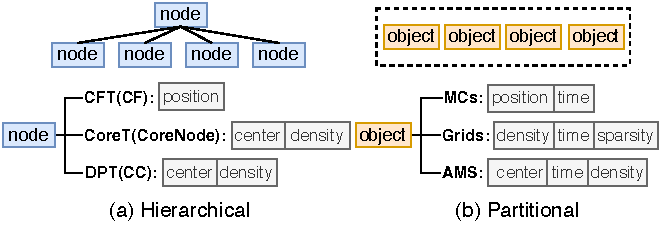
\includegraphics[width=0.5\textwidth]{Figures/DesignAspects/SummarizingDataStructure.pdf}
\caption{Six Types of Summarizing Data Structure in \algo.}
\label{fig:data_structure}
\end{figure}

\subsection{Summarizing Data Structure}
\label{sec:summarizing_data_structure}
In \algo, the summarizing data structure plays a critical role in providing a compact representation of the data points within the stream. This abstraction helps to enhance computational efficiency while maintaining a low memory footprint. Depending on the clustering needs, \algo offers two categories of summarizing data structures: the hierarchical category and the partitional category.

\subsubsection{Hierarchical Summarizing Data Structure}
\label{subsec:hierarchical}
Hierarchical data structures are primarily used in \algo when the data streams display inherent hierarchies or when the data can be logically grouped into a tree structure. As shown in Figure~\ref{fig:data_structure}(a), three types of hierarchical data structures are supported in \algo: Clustering Feature Tree (\CFT), Coreset Tree (\CoreT), and Dependency Tree (\DPT).

\textbf{Clustering Feature Tree (\CFT).}
\label{subsec:cf-tree}
\CFT~\cite{BIRCH:96} represents a classic yet efficient choice for hierarchical data representation in \algo. Its structure supports a broad range of basic operations required in stream clustering, such as distance calculation and cluster updating, thus providing a solid foundation for further complex manipulations.

\textbf{Coreset Tree (\CoreT).}
\label{subsec:CT}
When the data stream is characterized by high volume and density variations, \algo employs \CoreT~\cite{StreamKM++:12} to extract a core subset for processing. Despite the necessity of full tree rebuilding during clustering, which could affect efficiency, the application of \CoreT in \algo helps in obtaining high-quality clusters from dense data streams.

\textbf{Dependency Tree (\DPT).}
\label{subsec:DPT}
\DPT~\cite{EDMStream:17} is \algo's choice for handling cluster evolution effectively. The tree structure of \DPT, specifically designed to adapt to evolving activities in the stream, ensures that \algo delivers high clustering accuracy even in dynamic environments.

\subsubsection{Partitional Summarizing Data Structure}
\label{subsec:partition}
Partitional data structures, as shown in Figure~\ref{fig:data_structure}(b), are beneficial when the data streams are best represented by flat, non-overlapping clusters. In \algo, these structures are used to effectively handle and categorize incoming data points into appropriate clusters. The algorithm supports three types of partitional data structures: Micro Clusters (\MCs), Grids (\Grids), and Augmented Meyerson Sketch (\MS).

\textbf{Micro Clusters (\MCs).} 
\label{subsec:MCs}
\MCs~\cite{Clustream:03} serve as a means to reduce the computational load by representing a group of closely related data points as a single entity. With the additional elements for summarizing timestamps for clusters' updates, \MCs enable \algo to accurately track real-time clustering activities, especially under cluster evolution.

\textbf{Grids (\Grids).}
\label{subsec:Grids}
\algo uses \Grids~\cite{DStream:2007} when efficiency is paramount. The structure eliminates the need for frequent distance calculations between new data and the grid, boosting performance. Additionally, the periodic removal of sparse grids optimizes resource usage, while its fixed position may limit accuracy in cases of frequent evolving activities.

\textbf{Augmented Meyerson Sketch (\MS).}
\label{subsec:meyerson_sketch}
The \MS~\cite{SL-KMeans:20} is utilized for summarizing clustering information with a limited number of data points. Though it can be cost-intensive due to the need for sketch reconstruction to adapt to evolving data streams, it is applicable in scenarios where the exact number of clusters is known a priori. This flexibility helps \algo to accommodate diverse clustering needs.

\begin{figure}[t]
\centering
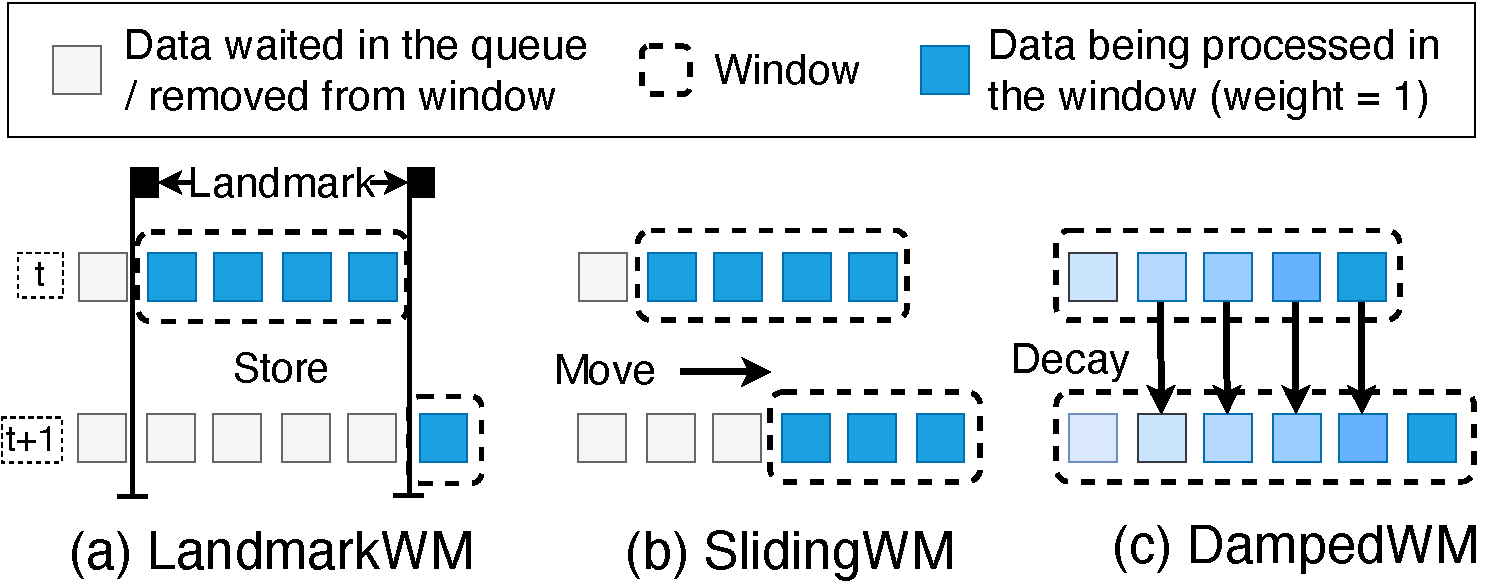
\includegraphics[width=0.5\textwidth]{Figures/DesignAspects/WindowModel.pdf}
\caption{Three Types of Window Model.}
\label{fig:window_model}
\end{figure}

\subsection{Window Model}
\label{sec:window_model}
In \algo, the window model determines the scope of the data stream that is under consideration for clustering at any given time. The selected window model influences how \algo can adapt to evolving data distributions and concept drifts. As illustrated in Figure~\ref{fig:window_model}, the three primary types of window models supported in \algo are the Landmark Window Model (\landmark), the Sliding Window Model (\sliding), and the Damped Window Model (\damped).

\subsubsection{Landmark Window Model}
\label{subsec:landmark}
In the \landmark~\cite{metwally2005duplicate}, the data stream is divided into fixed-size windows starting from a predefined landmark point. This model aids in detecting concept drifts and periodic patterns in the data by facilitating comparisons of clustering results across different windows. The primary challenge with the \landmark lies in deciding the spacing between landmarks, which has an impact on clustering accuracy and efficiency.

\subsubsection{Sliding Window Model}
\label{subsec:sliding}
The \sliding~\cite{zhou2008tracking,SL-KMeans:20} focuses on a fixed-size window encompassing the most recent data points for clustering. As new data points are processed, the oldest ones are discarded, ensuring that the algorithm remains responsive to the latest trends in the data. This model may, however, compromise clustering accuracy, particularly when the window size is small.

\subsubsection{Damped Window Model}
\label{subsec:damped}
The \damped~\cite{cao2006density,DStream:2007} assigns exponentially decaying weights to data points based on their age, giving precedence to recent data points while still considering older ones. This approach enables smoother adaptation to evolving data distributions. The \damped model is susceptible to certain stream characteristics, such as outlier effects, due to its predefined decay function parameters.

\begin{figure}
    \centering
    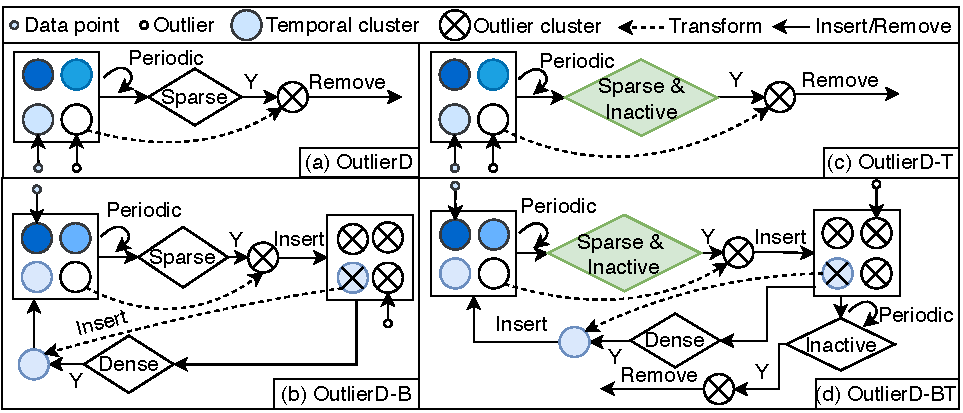
\includegraphics[width=1\linewidth]{Figures/DesignAspects/OutlierDetection.pdf}
    \caption{Four Types of Outlier Detection Mechanisms.}    \label{fig:outlier_detection_mechanisms}
\end{figure}
\subsection{Outlier Detection Mechanism}
\label{sec:outlier_detection}
Outlier detection mechanisms are optional design aspects in \algo that contribute to ensuring the quality of clustering results by identifying data points that deviate significantly from the overall data distribution. The two independent enhancements for this mechanism are the use of a buffer and a timer. We provide five variations, including not using any outlier detection mechanism (\nod). The other four variations are illustrated in Figure~\ref{fig:outlier_detection_mechanisms}.

\subsubsection{Basic Outlier Detection}
\label{subsec:detection}
As depicted in Figure~\ref{fig:outlier_detection_mechanisms}(a), the Basic Outlier Detection (\od) periodically identifies and removes low-density temporal clusters, improving clustering accuracy without significantly impacting efficiency~\cite{Clustream:03,DStream:2007}. Outlier detection methods can be further categorized into distance-based, density-based, and grid-based approaches, each suited to particular data stream characteristics.

\subsubsection{Outlier Detection with Buffer}
\label{subsec:buffer}
The Buffer variant (\buffer) retains potential outliers in a buffer for possible future clustering, as shown in Figure~\ref{fig:outlier_detection_mechanisms}(b)~\cite{DenStream:06,EDMStream:17}. This approach improves the overall clustering performance by keeping the temporal clusters representative of the underlying data distribution and preventing the immediate incorporation of potential outliers.

\subsubsection{Outlier Detection with Timer}
\label{subsec:timer}
The Timer variant (\timer) uses a timer mechanism, as illustrated in Figure~\ref{fig:outlier_detection_mechanisms}(c), to evaluate the activity of temporal clusters before transforming them into outlier clusters. This method enhances the robustness of the outlier detection process and the overall accuracy of the clustering results. The trade-off is an increase in algorithmic complexity and the risk of preserving noisy clusters.

\subsubsection{Outlier Detection with Buffer and Timer}
\label{subsec:buffertimer}
As depicted in Figure~\ref{fig:outlier_detection_mechanisms}(d), the combined Buffer and Timer variant (\buffertimer) retains outlier clusters in a buffer and uses a timer to evaluate their activity before transforming them into outlier clusters. Although this method improves the clustering accuracy, it increases the time required for buffer maintenance.

\subsection{Refinement Strategy}
\label{sec:refinement_strategy}
The refinement strategy, an optional design aspect, helps to maintain the adaptability of \dsc algorithms to evolving data distributions and concept drifts by updating the clustering model with new data points. Depending on computational efficiency, clustering accuracy, and adaptability to data distribution changes, there are three strategies available: \norefinement, \oneshotRefinement, and \incrementalRefinement.

\subsubsection{No Refinement}
\label{sec:no_refinement}
The \norefinement strategy, as depicted in Figure~\ref{fig:refinement} (a), outputs the temporal clusters $C$ as the final results without further refinement. This strategy saves computational resources but may lower the clustering accuracy when handling evolving data distributions or concept drifts.

\subsubsection{One-shot Refinement}
\label{sec:oneshot_refinement}
The \oneshotRefinement strategy (Figure~\ref{fig:refinement} (b)) performs model refinement less frequently to balance computational efficiency and clustering accuracy. This strategy is effective when computational resources are limited or the data stream changes gradually, allowing infrequent model updates.

\subsubsection{Incremental Refinement}
\label{sec:incremental_refinement}
The \incrementalRefinement strategy (Figure~\ref{fig:refinement} (c)) updates the clustering model continuously as new data points arrive. This keeps the model current and adaptable but may increase computational overhead. The trade-off is improved clustering accuracy at the cost of computational complexity.

\begin{figure}
    \centering
    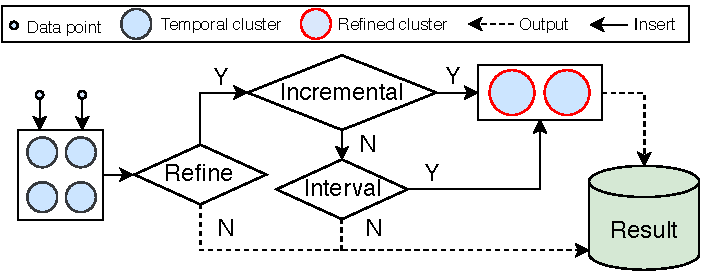
\includegraphics[width=0.45\textwidth]{Figures/DesignAspects/OfflineRefinementStrategy.pdf}
    \caption{Refinement Strategies.}
    \label{fig:refinement}
\end{figure}
